% All labels/arrows are vector graphics. Images are genuine recorded UI replays.
% Set \LabFigureFrame to 0 to compare the otherwise identical unframed variant.
\providecommand{\LabFigureFrame}{1}
\begin{tikzpicture}[x=1mm,y=1mm,>=Latex,
  every node/.style={inner sep=0,align=left,font=\fontsize{8.4}{9.5}\selectfont},
  flow/.style={-{Latex[length=3.1mm,width=2.8mm]},draw=accent,
    line width=2.2pt,line cap=round},
  outline/.style={draw=rulegray,line width=.55pt,rounded corners=2mm}]
\path[use as bounding box] (0,0) rectangle (180,82);
\ifnum\LabFigureFrame=1
  \draw[draw=rulegray!75,line width=.6pt,rounded corners=3mm,fill=pale!55] (.2,.2) rectangle (179.8,81.8);
\fi
\node[anchor=west,font=\fontsize{9}{10}\selectfont\bfseries,text=accent] at (5,77.5)
  {LABOPSBENCH: A SHARED EVALUATION LOOP};

% One shared engine; the inset contains two illustrative, independently run cases.
\draw[outline,fill=white] (5,18.5) rectangle (96,73);
\node[anchor=north west,font=\fontsize{10}{11}\selectfont\bfseries] at (8,70.5)
  {Laboratory Simulator (Engine)};
\node[anchor=north west,font=\fontsize{8.5}{9.5}\selectfont\bfseries,text=accent] at (8,65.2)
  {Example Scenarios (2 of 14)};
\path[fill=pale,rounded corners=1.5mm] (7.5,24) rectangle (93.5,61.2);
\node[anchor=north west,font=\fontsize{8.3}{9.2}\selectfont\bfseries] at (9,59.9)
  {(a) Two-Bay Cell};
\node[anchor=north west,font=\fontsize{8.3}{9.2}\selectfont\bfseries] at (48,59.9)
  {(b) 32-Station Hall};
\node[anchor=north west] at (9,56.3846)
  {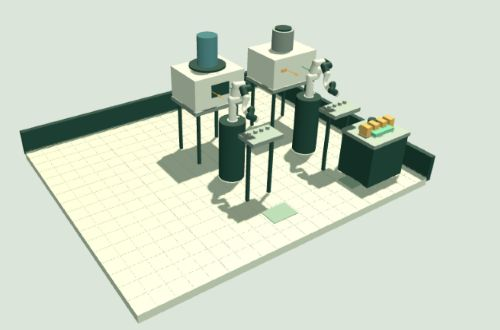
\includegraphics[width=35mm]{assets/lab-runtime-angle.jpg}};
% Exact viewport crop in TikZ: x=190..710, y=175..475 of a 1275x717 screenshot.
% No objects, colours or recorded geometry are added to the screenshot.
\begin{scope}[shift={(48,31)}]
  \clip (0,0) rectangle (44,25.3846);
  \node[anchor=north west] at (-16.076923,40.192307)
    {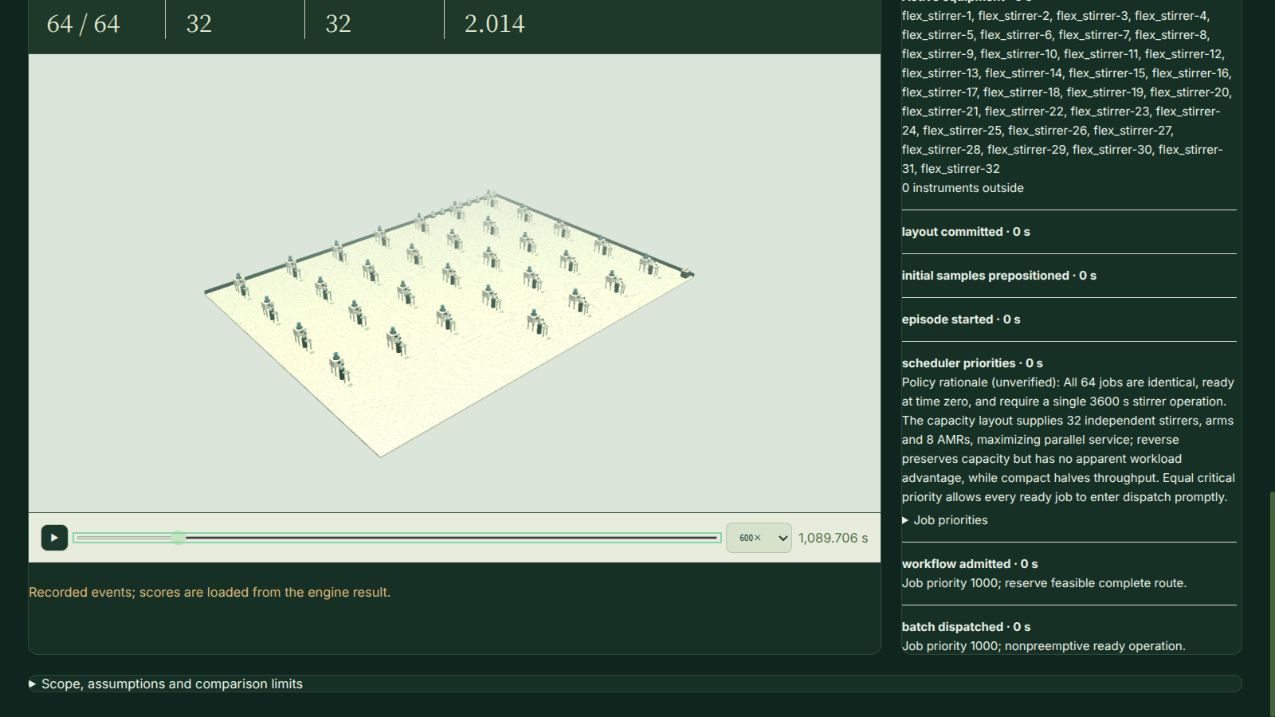
\includegraphics[width=107.884615mm]{assets/lab-runtime-large.png}};
\end{scope}
\node[anchor=north west,font=\fontsize{8}{9}\selectfont] at (9,30)
  {2 active instruments, 22 jobs\\$4\times3.4$ m; 34 stored outside};
\node[anchor=north west,font=\fontsize{8}{9}\selectfont] at (48,30)
  {32 instruments, 32 arms\\$32\times24$ m; 64 jobs, 8 AMRs};
\node[anchor=west,font=\fontsize{8.2}{9}\selectfont] at (8,21.5)
  {Validate $\rightarrow$ dispatch $\rightarrow$ advance simulated time};

% Observation -> policy -> action forms the right side of the loop.
\draw[outline,fill=white] (104,53) rectangle (175,73);
\node[anchor=north west,font=\fontsize{8.8}{9.8}\selectfont\bfseries] at (107,70.5)
  {INPUT: Observation at $t_k$};
\node[anchor=north west] at (107,65.5)
  {\textbf{Jobs:} arrivals, dependencies, durations\\
   \textbf{Lab:} layout, occupancy, resource limits\\
   \textbf{Menu:} public candidates; prior receipts};
\draw[fill=accent,draw=accent,rounded corners=2mm] (111,39.5) rectangle (168,48.5);
\node[text=white,anchor=center,align=center,font=\fontsize{10.4}{11}\selectfont\bfseries] at (139.5,45.2)
  {AI AGENT / ALGORITHM};
\node[text=white,anchor=center,font=\fontsize{8}{9}\selectfont] at (139.5,41.4)
  {Select equipment and prioritize jobs};
\draw[outline,fill=white] (104,20.5) rectangle (175,35);
\node[anchor=north west,font=\fontsize{8.8}{9.8}\selectfont\bfseries] at (107,32.8)
  {OUTPUT: Structured Decision};
\node[anchor=north west] at (107,28)
  {$t=0$: design candidate $+$ job priorities\\
   Later: priorities $+$ keep / allowed exchange};
\draw[flow] (96,63)--(104,63);
\draw[flow] (139.5,53)--(139.5,48.5);
\draw[flow] (139.5,39.5)--(139.5,35);
\draw[flow] (104,25)--(96,25);

% Timeline is part of the figure, below the loop and inside its outer frame.
\draw[rulegray!55,line width=.4pt] (5,16.3)--(175,16.3);
\node[anchor=north west,font=\fontsize{8.2}{9.2}\selectfont\bfseries] at (5,14.2)
  {Decision\\Timing};
\draw[->,rulegray,line width=.7pt] (30,12.7)--(174,12.7);
\foreach \x/\lab in {34/{$t=0$},74/{$1{,}800$ s},114/{$3{,}600$ s}}{
  \fill[accent] (\x,12.7) circle (.75);
  \node[anchor=north,align=center,font=\fontsize{8.2}{9}\selectfont] at (\x,10.9){\lab};
}
\node[anchor=center,fill=pale!55,inner sep=.8mm] at (137,12.7){$\cdots$};
\fill[accent] (159,12.7) circle (.75);
\node[anchor=north,align=center,font=\fontsize{8.2}{9}\selectfont] at (159,10.9){Completion};
\node[anchor=south west,font=\fontsize{8}{9}\selectfont] at (5,3)
  {Calls pause the clock; at most 32 submissions including $t=0$. Score: total completion time (makespan).};
\end{tikzpicture}
